You have an Art History exam approaching, but you have been paying more attention to
informatics at school than to your art classes! You will need to write a program to take the
exam for you.

The exam will consist of several paintings. Each painting is an example of one of four
distinctive styles, numbered 1, 2, 3 and 4.

Style 1 contains neoplastic modern art. For example:

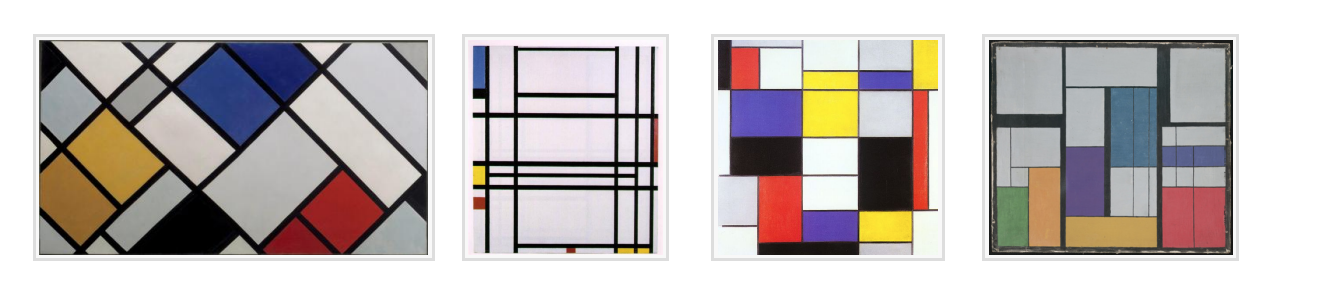
\includegraphics[scale=0.8]{artclass1.png}

Style 2 contains impressionist landscapes. For example:

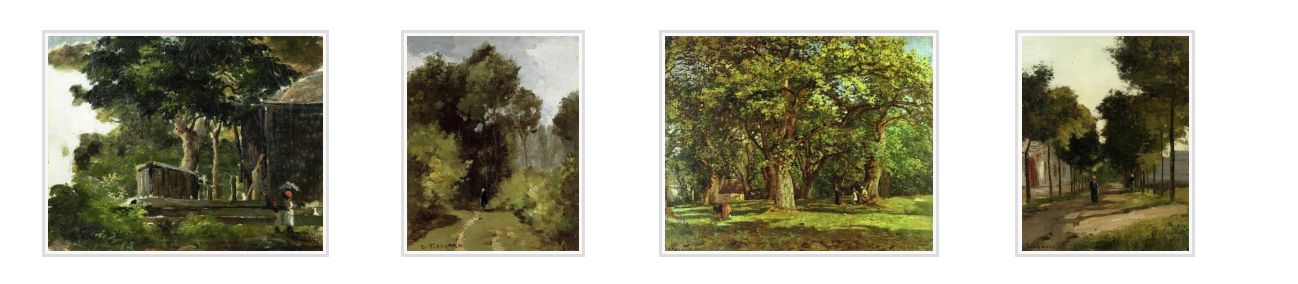
\includegraphics[scale=0.8]{artclass2.png}

Style 3 contains expressionist action paintings. For example:

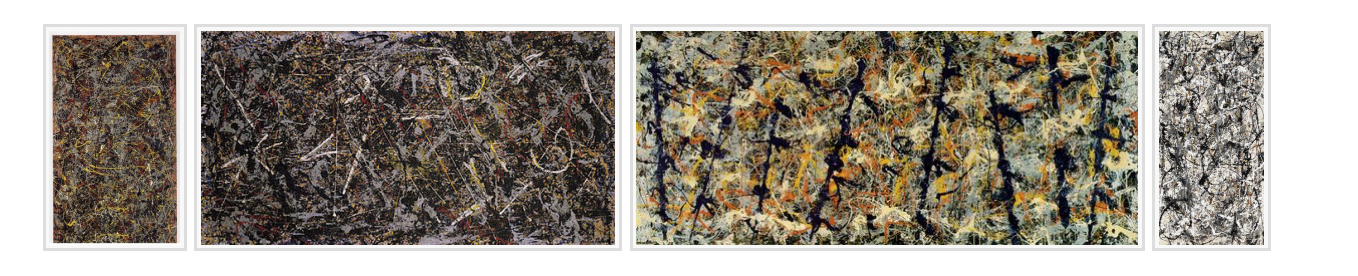
\includegraphics[scale=0.8]{artclass3.png}

Style 4 contains colour field paintings. For example:

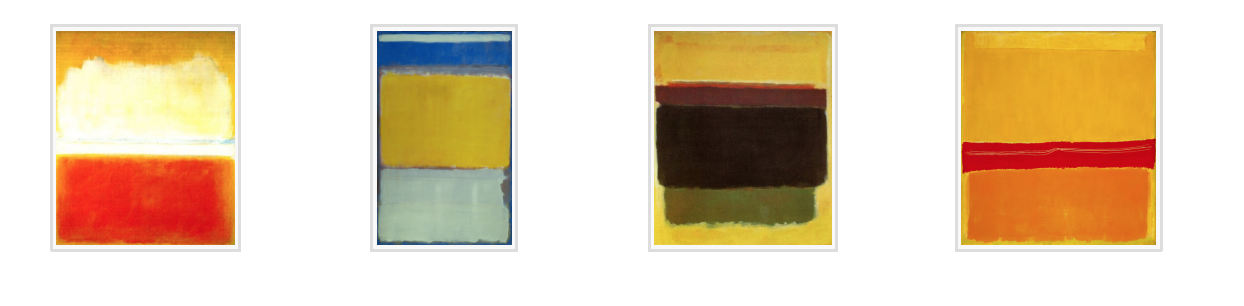
\includegraphics[scale=0.8]{artclass4.png}

Your task is, given a digital image of a painting, to determine which style the painting
belongs to.

The IOI judges have collected many images in each style. Nine images from each style
have been chosen at random and included in the task materials you can download in problem materials section, so that you can examine them by hand and use them for testing. Each of them is given in two forms --- jpeg picture, you can view, and text format, which would be given to your program. The remaining images will be given to your program during grading.

The image will be given as an $H \times W$ grid of pixels. The rows of the image are numbered
$0, \dots, H ­- 1$ from top to bottom, and the columns are numbered $0, \dots, W ­- 1$ from left to right.

The pixels are described using two­dimensional arrays $R$, $G$ and $B$, which give the
amount of red, green and blue respectively in each pixel of the image. These amounts range
from $0$ (no red, green or blue) to $255$ (the maximum amount of red, green or blue).

You should submit a file that implements the function \t{style()} on C/C++, as follows:

\t{int style(int H, int W, int R[500][500], int G[500][500], int B[500][500]);}

This function should determine the style of the image.

Parameters:
\begin{itemize}
\item $H$: The number of rows of pixels in the image.
\item $W$: The number of columns of pixels in the image.
\item $R$: A two­dimensional array of size $H \times W$, giving the amount of red in each pixel of the image.
\item $G$: A two­dimensional array of size $H \times W$, giving the amount of green in each pixel of the image.
\item $B$: A two­dimensional array of size $H \times W$, giving the amount of blue in each pixel of the image.
\item \textit{Returns}: The style of the image, which must be $1$, $2$, $3$ or $4$, as described above.
\end{itemize}

Each array element $R[i][j]$, $G[i][j]$ and $B[i][j]$ refers to the pixel in row $i$ and
column $j$, and will be an integer between $0$ and $255$ inclusive.